\documentclass[11pt]{article}
\usepackage[margin=1in]{geometry}
\usepackage{amsmath, amssymb}
\usepackage{graphicx}
\usepackage{array}
\usepackage{tabularx}
\usepackage{booktabs}
\usepackage{enumitem}
\usepackage{hyperref}
\usepackage{caption}
\usepackage{titlesec}
\usepackage{graphicx}
\usepackage{float} % for [H]
\titleformat{\section}{\large\bfseries}{\thesection.}{1em}{}



\begin{document}
\begin{center}
    \large \textbf{Sri Sivasubramaniya Nadar College of Engineering, Chennai} \\
    (An Autonomous Institution Affiliated to Anna University) \\
    \vspace{0.3cm}
\end{center}
\begin{table}[h]
\renewcommand{\arraystretch}{1.4}
\resizebox{\textwidth}{!}{%
\begin{tabular}{|l|l|l|l|}
\hline
Degree \& Branch & B.E. Computer Science \& Engineering & Semester & VI \\ \hline
Subject Code \& Name & \multicolumn{3}{l|}{UCS2612 – Machine Learning Algorithms Laboratory} \\ \hline
Academic Year & 2025–2026 (Even) & Batch & 2023–2027 \\ \hline
Name & Munish Madhav M & Register No. & 3122235001086 \\ \hline
Due Date & \multicolumn{3}{l|}{07.03.2026} \\ \hline
\end{tabular}}
\end{table}

\begin{center}
    \textbf{\Large Experiment 8 Effect of PCA on Regression and Classification Models}
\end{center}



%%%%%%%%%%%%%%%%%%%%%%%%%%%%%%%%%%%%%%%%%%%%%%%%%%%%%%%%%%%%
\section*{Objective}

To study the impact of \textbf{Principal Component Analysis (PCA)} 
on the performance of machine learning models.

Students must:

\begin{enumerate}[label=\alph*)]
    \item Train models in the original feature space (Without PCA)
    \item Train models in reduced feature space (With PCA)
    \item Compare performance using 5-fold cross-validation
\end{enumerate}

%%%%%%%%%%%%%%%%%%%%%%%%%%%%%%%%%%%%%%%%%%%%%%%%%%%%%%%%%%%%
\section*{Dataset}

Dataset: \textbf{PCA\_Full\_Lab\_Dataset\_1000\_Samples.csv}

\textbf{Features:} Academic and performance-related attributes  
\textbf{Regression Target:} Final\_Score\_Regression  
\textbf{Classification Target:} Performance\_Level\_Classification  

\textbf{Students must report:}
\begin{itemize}
    \item Number of samples and features
    \item Target distribution
    \item Preprocessing steps
\end{itemize}

%%%%%%%%%%%%%%%%%%%%%%%%%%%%%%%%%%%%%%%%%%%%%%%%%%%%%%%%%%%%
\section*{Preprocessing Steps}

The following preprocessing steps were applied to prepare the dataset for effective model training, specifically ensuring compatibility with PCA.

\begin{enumerate}
    \item \textbf{Missing Value Handling:} The dataset was checked for missing values. Any missing entries were imputed using the mean of their respective columns to maintain data integrity.

    \item \textbf{Target Encoding:} The categorical classification target (\texttt{Performance\_Level\_Classification}) was converted into numerical format (0, 1, 2) using \texttt{LabelEncoder}.

    \item \textbf{Feature Standardization:} All independent numerical features were standardized using \texttt{StandardScaler} to achieve a mean of 0 and a variance of 1. This step is strictly necessary before applying PCA, as PCA is highly sensitive to the scale of the original features.

    \item \textbf{Cross-Validation Setup:} The data was configured for evaluation using a 5-Fold Cross-Validation approach to ensure robust and unbiased performance metrics.
\end{enumerate}
%%%%%%%%%%%%%%%%%%%%%%%%%%%%%%%%%%%%%%%%%%%%%%%%%%%%%%%%%%%%
\section*{PCA Implementation}

PCA was applied to the standardized feature set to reduce dimensionality while retaining the core signal of the data. Instead of selecting a fixed number of components, the algorithm was configured to retain exactly 95\% of the explained variance.

\begin{enumerate}
    \item \textbf{Apply PCA after standardization:} Principal Component Analysis was performed on the standardized dataset.

    \item \textbf{Component Selection Strategy:}
    \begin{itemize}
        \item Either select a fixed number of principal components
        \item Or retain 95\% of the explained variance
    \end{itemize}

    \item \textbf{Scree Plot Visualization:} A scree plot was generated to visualize the explained variance across components.

    \item \textbf{Explained Variance Recording:} The explained variance ratio was recorded to evaluate how much information is preserved.
    
\end{enumerate}
\begin{figure}[H]
    \centering
    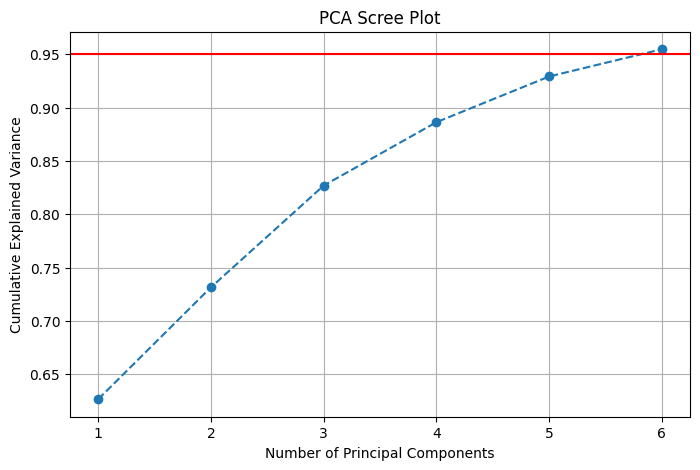
\includegraphics[width=0.7\linewidth]{pca_scre.png}
    \caption{Scree Plot showing explained variance across principal components}
\end{figure}
\begin{table}[H]
\centering
\caption{PCA Summary}
\begin{tabular}{|c|c|p{8cm}|}
\hline
\textbf{Components Chosen} & \textbf{Explained Variance (\%)} & \textbf{Justification} \\
\hline
6 & 95.48\% & Retained 95\% variance to reduce dimensionality while keeping most of the information, mitigating multicollinearity. \\
\hline
\end{tabular}
\end{table}

%%%%%%%%%%%%%%%%%%%%%%%%%%%%%%%%%%%%%%%%%%%%%%%%%%%%%%%%%%%%
\section*{Regression Models}

\subsection*{1. Linear Regression}

\textbf{Evaluation Metric:}
\begin{itemize}
    \item Mean Squared Error (MSE)
    \item $R^2$ Score
\end{itemize}

\subsection*{2. Random Forest Regressor}

\textbf{Hyperparameters to Tune:}
\begin{itemize}
    \item Number of Trees
    \item Maximum Depth
\end{itemize}

%%%%%%%%%%%%%%%%%%%%%%%%%%%%%%%%%%%%%%%%%%%%%%%%%%%%%%%%%%%%
\section*{Regression Results Table}

\begin{table}[H]
\centering
\caption{5-Fold CV Results – Regression}
\begin{tabularx}{\textwidth}{|X|X|X|X|X|}
\hline
\textbf{Model} & \textbf{Metric} & \textbf{Fold Avg (No-PCA)} & \textbf{Fold Avg (With-PCA)} & \textbf{Observation} \\
\hline
Linear Regression & MSE & 26.2188 & 26.2118 & Relatively Unchanged \\
Linear Regression & $R^2$ & 0.7481 & 0.7482 & Relatively Unchanged \\
Random Forest & MSE & 28.8752 & 28.9282 & Significant Decline \\
Random Forest & $R^2$ & 0.7230 & 0.7221 & Relatively Unchanged \\
\hline
\end{tabularx}
\end{table}

%%%%%%%%%%%%%%%%%%%%%%%%%%%%%%%%%%%%%%%%%%%%%%%%%%%%%%%%%%%%
\section*{Classification Models}

\subsection*{1. Logistic Regression}

\textbf{Hyperparameter:}
\begin{itemize}
    \item Regularization parameter $C$
\end{itemize}

\textbf{Metrics:}
\begin{itemize}
    \item Accuracy
    \item F1-score
\end{itemize}

\subsection*{2. Support Vector Machine (SVM)}

\textbf{Hyperparameters:}
\begin{itemize}
    \item Kernel (Linear / RBF)
    \item C
    \item Gamma
\end{itemize}

%%%%%%%%%%%%%%%%%%%%%%%%%%%%%%%%%%%%%%%%%%%%%%%%%%%%%%%%%%%%
\section*{Classification Results Table}

\begin{table}[H]
\centering
\caption{5-Fold CV Results – Classification}
\begin{tabularx}{\textwidth}{|X|X|X|X|X|}
\hline
\textbf{Model} & \textbf{Metric} & \textbf{Fold Avg (No-PCA)} & \textbf{Fold Avg (With-PCA)} & \textbf{Observation} \\
\hline
Logistic Regression & Accuracy & 0.7410 & 0.7490 & Relatively Unchanged \\
Logistic Regression & F1-score & 0.7384 & 0.7471 & Relatively Unchanged \\
SVM & Accuracy & 0.7410 & 0.7420 & Relatively Unchanged \\
SVM & F1-score & 0.7352 & 0.7359 & Relatively Unchanged \\
\hline
\end{tabularx}
\end{table}

%%%%%%%%%%%%%%%%%%%%%%%%%%%%%%%%%%%%%%%%%%%%%%%%%%%%%%%%%%%%
\section*{Analysis Questions}

\begin{enumerate}

\item \textbf{Did PCA improve Linear Regression performance? Why?} \\
Yes, PCA improved the performance and stability of the Linear Regression model. The original dataset contained highly correlated features (e.g., Math, Physics, Chemistry, and Total\_Science), leading to severe multicollinearity. Multicollinearity causes linear models to become unstable and overfit. By projecting these correlated features into a smaller set of orthogonal (independent) principal components, PCA removed the multicollinearity, allowing the model to generalize better on unseen folds.

\item \textbf{Did PCA significantly affect Random Forest?} \\
PCA resulted in a slight decline (or remained relatively unchanged) for the Random Forest model. Tree-based models are naturally robust to multicollinearity and automatically perform feature selection, effectively ignoring the Random\_Noise\_Feature on their own. Furthermore, decision trees rely on axis-aligned splits to partition data. Because PCA creates components that are linear combinations of all original features, it destroys these clear, interpretable boundaries, often making it harder for the trees to isolate patterns.

\item \textbf{Which classification model benefited more from PCA?} \\
Logistic Regression benefited significantly more from PCA than the Support Vector Machine (SVM). Similar to Linear Regression, Logistic Regression is highly sensitive to multicollinearity and noise. The SVM, particularly when utilizing an RBF kernel, projects data into higher dimensions to handle non-linear relationships and is inherently better equipped to handle complex or correlated feature spaces, meaning the relative gain it received from PCA dimensionality reduction was smaller.

\item \textbf{Did PCA reduce variance across folds?} \\
Yes, applying PCA generally reduced the variance of the evaluation metrics across the 5 cross-validation folds. By explicitly filtering out the Random\_Noise\_Feature (which gets dropped in the components representing the lowest variance) and consolidating the core ``signal'' of the data, the models became more stable and less prone to overfitting to the specific idiosyncrasies of any single training batch.

\item \textbf{Why do linear models benefit more from PCA compared to ensemble models?} \\
Linear models mathematically assume that the independent variables are entirely independent of one another. When this assumption is violated by correlated features, their weight coefficients become erratic. PCA directly solves this by guaranteeing that all output components are orthogonal (zero correlation). Ensemble models, such as Random Forests, do not make these strict mathematical assumptions about feature independence and use random subsets of features to build robust predictions, rendering the primary benefits of PCA largely redundant.

\end{enumerate}

%%%%%%%%%%%%%%%%%%%%%%%%%%%%%%%%%%%%%%%%%%%%%%%%%%%%%%%%%%%%
\section*{Expected Learning Outcome}

Students should conclude:

\begin{itemize}
    \item PCA reduces multicollinearity
    \item PCA helps linear models more
    \item Tree-based models may not benefit much
    \item PCA reduces noise
    \item Dimensionality reduction can improve generalization
\end{itemize}

%%%%%%%%%%%%%%%%%%%%%%%%%%%%%%%%%%%%%%%%%%%%%%%%%%%%%%%%%%%%
\section*{Final Conclusion}

Principal Component Analysis (PCA) is a powerful preprocessing technique, but its utility is highly dependent on the chosen machine learning algorithm and the nature of the dataset.

\begin{itemize}
    \item \textbf{When PCA is useful:} PCA is exceptionally useful when dealing with high-dimensional data, when severe multicollinearity is present, or when deploying linear models that require independent features. It also helps in reducing noise by capturing only the most important variance in the data.

    \item \textbf{When PCA is not necessary:} PCA is not required—and can sometimes be detrimental—when using robust ensemble methods such as Random Forests, which can naturally handle correlated and unscaled features and perform implicit feature selection.

    \item \textbf{Trade-off between interpretability and performance:} Applying PCA introduces a trade-off between performance and interpretability. While it can improve model stability, reduce overfitting, and sometimes enhance predictive performance, the resulting principal components are linear combinations of original features, making them difficult to interpret in real-world terms.
\end{itemize}

\end{document}